In this chapter the test results of the tests that were taken to gain insight of the different system models and their performances are discussed.
First a general analysis is made by plotting the whole estimated flight as well a table which displays the errors of the different estimated values which were taken from multiple simulation cycles.
For this all estimations have been made with a mean acceleration offset of $ -1.31 m/s^2$  which was taken out of measurements from a test flight.
Also for the general analysis a perfectly linear temperature gradient of $-0.0065 °/m$ was used.
After that the different problematic properties of each system model is discussed in detail.
At the end the best system from the first tests has been further tested under different circumstances.


\section{Point Mass}
The first system model to test was the simple point mass model as described in chapter \ref{ch:Approach}.
While this implementation is a simple version it does already work surprisingly good.
In Figure \ref{fig:PointMassPerformance} the overall performance of its estimation of the different values can be seen.


\begin{figure}[h!]
 \centering
 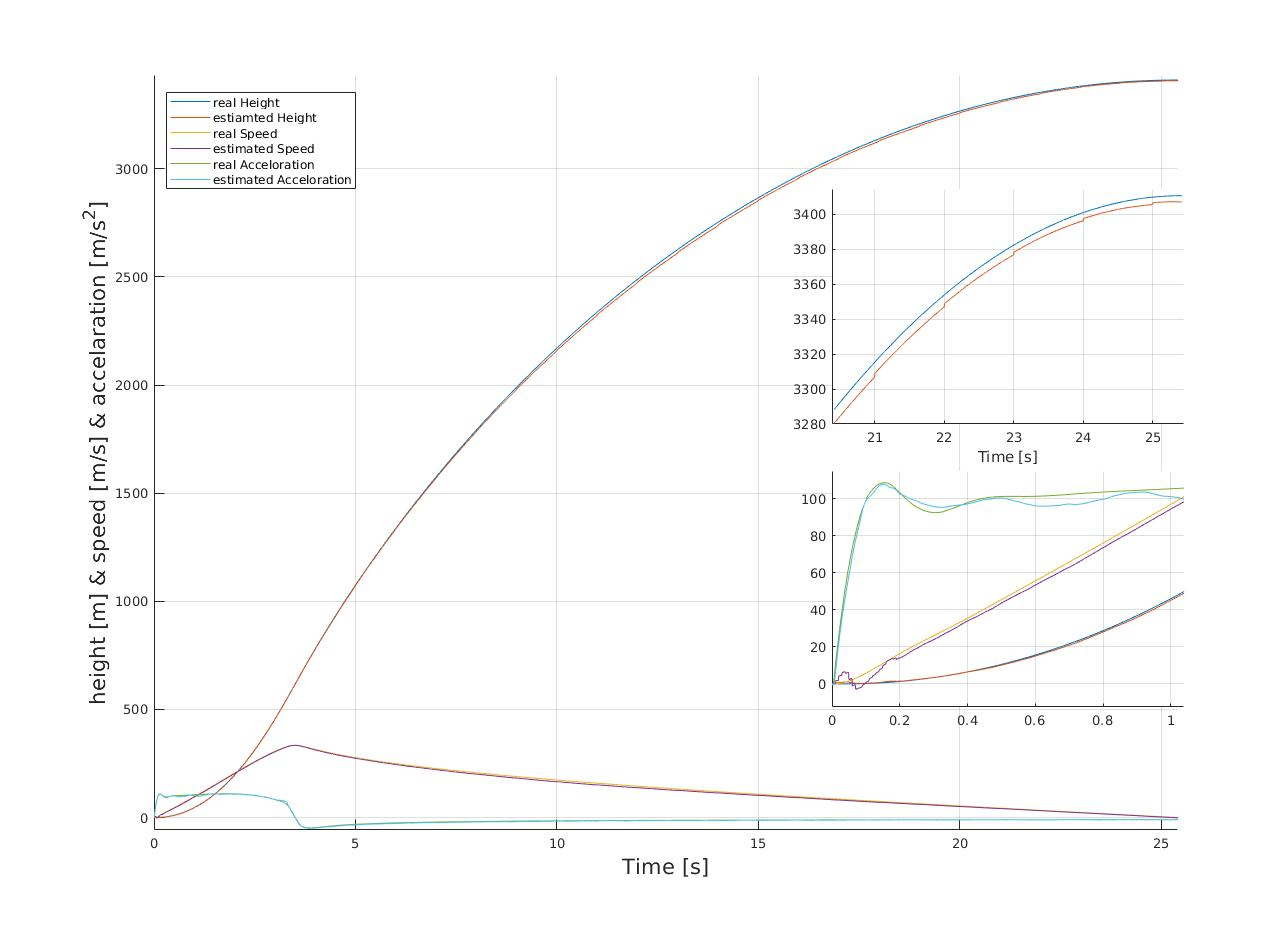
\includegraphics[width=.8\textwidth]{./Pictures/PointMassPerformance.jpg}
 % PointMassPerformance.jpg: 0x0 pixel, 300dpi, 0.00x0.00 cm, bb=
 \caption{The performance of the point mass system model over time}
 \label{fig:PointMassPerformance}
\end{figure}

Especially the first second (lower right corner) and the last five seconds (upper right corner) are interesting.
It can be seen that the system does not really have a settling time at all,
because the height is estimated at the minimal error at the beginning of the estimation.
On the other hand the speed needs around 0.2 seconds to settle on the right value.
Also a clear error on the estimation of the error can be seen after the speed has settled,
this is due to the fact that the estimator can trust the GPS and pressure measurements much more at the beginning than the acceleration measurements.
Therefore the estimator does adapt the acceleration estimation on the height and speed estimation at the start and not the other way around.
In the last five second it can be seen that the height is far more off as it was at the start.
Also the steps the estimation makes there are coming from the GPS measurements.
In addition Table \ref{tab:ErrorPointMass} shows the maximum, minimum, mean and median error of the estimated values.

\begin{table}[h!]
\centering
\begin{tabular}{cccccc}
\hline
\multicolumn{1}{|c|}{State Variable} & \multicolumn{1}{c|}{Unit} & \multicolumn{1}{c|}{Max} & \multicolumn{1}{c|}{Min} & \multicolumn{1}{c|}{Mean} & \multicolumn{1}{c|}{Median} \\ \hline
Height                            & $m$                         & 20.05                  & 1.18e-05                 & 4.72                    & 2.20                      \\
Speed                             & $m/s$                       & 3.42e+03               & 0                        & 3.40                    & 2.43                      \\
Acceleration                       & $m/s^2$   			& 17.79                  & 2.55e-05                 & 1.67                    & 1.55
\end{tabular}
\caption{Error of estimated state variables}
\label{tab:ErrorPointMass}
\end{table}

The most interesting value is the median from the height error because it is free from outliers.
It shows that the height error is with 2.2 meter slightly above the aimed 2 meter.
The 20 meter maximum error occurs around second 15 of the flight just before a new GPS measurement comes in.
At this time stamp the offset on the acceleration measurements does have a greater impact because the real value is in comparison to the start rather small.
In addition the height does change more between two GPS measurements than it does at the end of the flight, therefore greater errors in the interpolation between can occur.
Additionaly the minimum speed error occurs at the beginning of the estimation loop where the speed still zero.


\subsection{Greater Offset}
It has to be said that this only works while no sensor has a bigger offset.
Therefore these values come at the cost that they are not that trustworthy,
because the system noise on the acceleration has to be set to a greater value to get those good estimations.
An additional factor is also the pitch angle which does hinder this estimation if it changes in a great manner.
This can be seen in Figure \ref{fig:PointMassErrorWithOffset} which shows the state estimation error with different offsets.

\begin{figure}[h!]
 \centering
 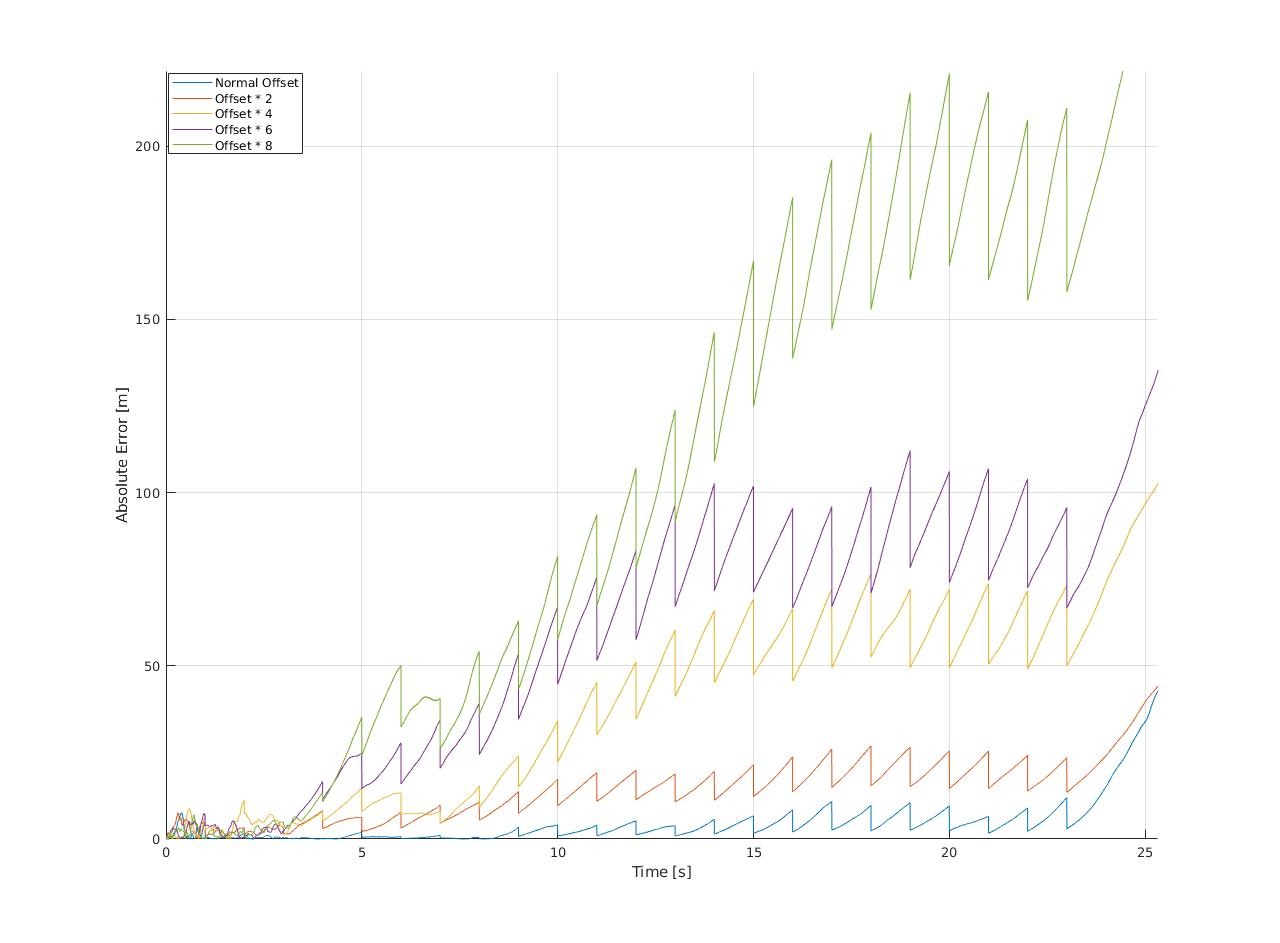
\includegraphics[width=.8\textwidth]{./Pictures/PointMassErrorWithOffset.jpg}
 % PointMassErrorWithOffset.jpg: 0x0 pixel, 300dpi, 0.00x0.00 cm, bb=
 \caption{Error during flight time with different offsets}
 \label{fig:PointMassErrorWithOffset}
\end{figure}


Table \ref{tab:PointMassPerformanceWithOffset} shows the mean and median of the error in the height depending on the offset on the accelerometer.

\begin{table}[h!]
\centering
\begin{tabular}{ccc}
\hline
\multicolumn{1}{|c|}{Offset} & \multicolumn{1}{|c|}{Mean}& \multicolumn{1}{|c|}{Median} \\ \hline
%
% & Mean & Median\\
Normal & 4.57 & 2.80\\
2 Times & 13.97 & 14.66\\
4 Times & 39.31 & 46.99\\
6 Times & 59.35 & 71.90\\
8 Times & 107.21 & 102.15
\end{tabular}
\caption{Error of the height in meter with changing offset}
\label{tab:PointMassPerformanceWithOffset}
\end{table}

This shows that the error which the estimator makes does rise exponentially.
So this is an issue which should be assessed by including an acceleration offset in the state vector.


\section{Point Mass with Acceleration Offset}
The overall performance of this system model can be seen in the figure \ref{fig:PointMassOffsetPerformance}.

\begin{figure}[h!]
 \centering
 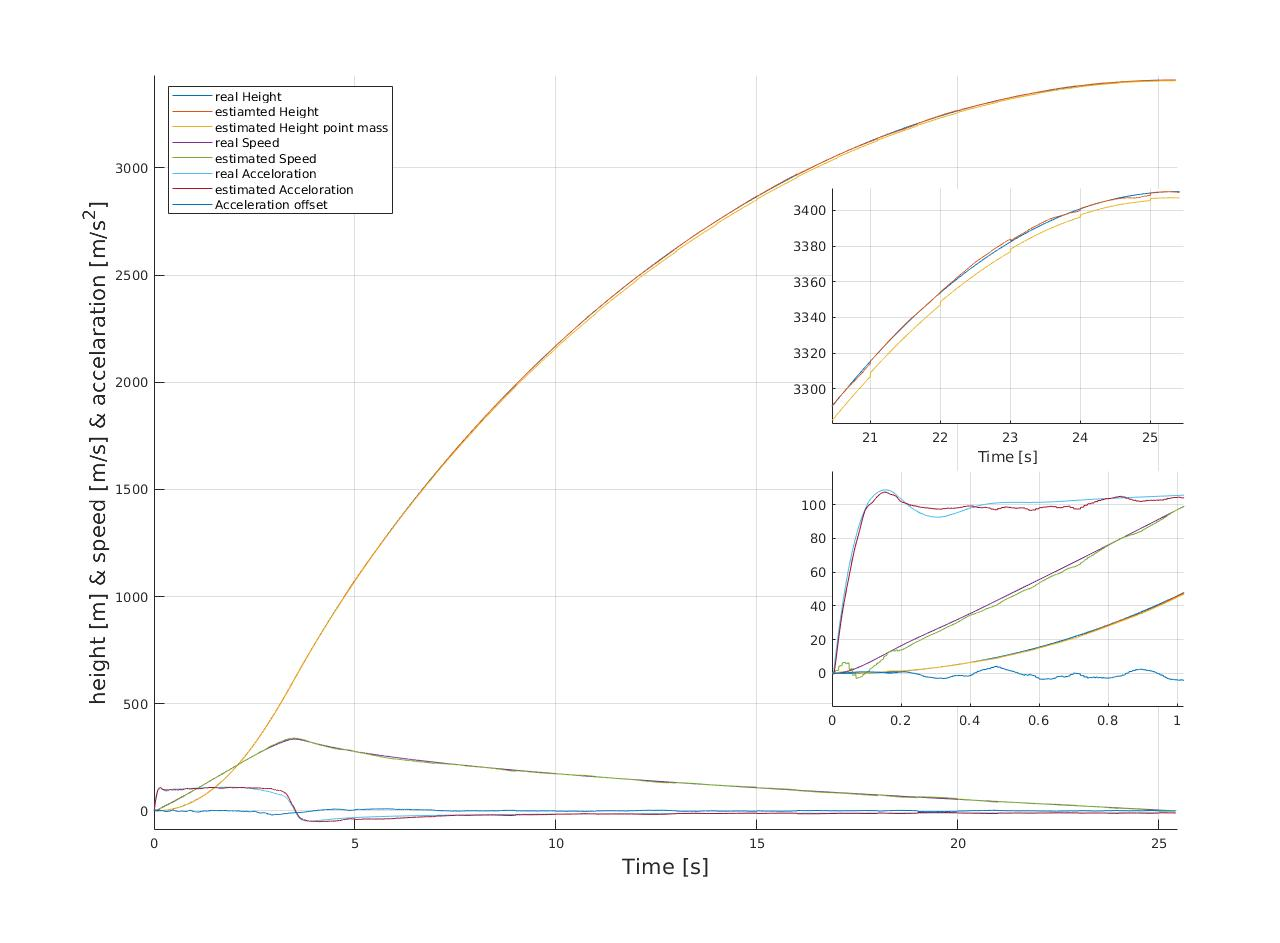
\includegraphics[width=.8 \textwidth]{./Pictures/PointMassOffsetPerformance.jpg}
 % PointMassOffsetPerformance.jpg: 0x0 pixel, 300dpi, 0.00x0.00 cm, bb=
 \caption{Performance of point mass with acceleration offset over time}
 \label{fig:PointMassOffsetPerformance}
\end{figure}

While the speed and height of it performs more or less the same way at the first second like the point mass system model,
a clear difference in the estimated acceleration can be seen.
This is possible due to the fact that the estimator can describe the difference in the system description between the speed and acceleration as the acceleration offset.
These dependencies can be seen after the settling of the speed where the estimator starts to change the acceleration offset value to adjust the acceleration.
The great advantage of this can be seen in the plot of the last five seconds of the height estimation (upper right plot).
Due to the better estimation of the acceleration over the whole time, the dependencies of the height on the acceleration is much more trustworthy.
When the rocket does rise at further height and the measurements of the barometers lose their accuracy,
the better acceleration measurements can be used to interpolate between the good GPS measurements.
This results in a much better height estimation at greater height.

\begin{table}[h!]
\centering
\begin{tabular}{cccccc}
\hline
\multicolumn{1}{|c|}{State Variable} & \multicolumn{1}{c|}{Unit} & \multicolumn{1}{c|}{Max} & \multicolumn{1}{c|}{Min} & \multicolumn{1}{c|}{Mean} & \multicolumn{1}{c|}{Median} \\ \hline
Height                            & $m$                         & 9.78                   & 2.98e-06                 & 1.33                    & 0.83                      \\
Speed                             & $m/s$                       & 78.79                  & 0                        & 3.18                    & 2.22                      \\
Acceleration                       & $m/s^2$   			& 165.87                  & 1.35e-05                 & 4.52                    & 2.64                     \\
Acceleration Offset                & $m/s^2$   			& 167.46                  & 2.66e-05                 & 4.44                    & 2.61
\end{tabular}
\caption{Error of estimated state variables point mass with acceleration offset}
\label{tab:ErrorPointMassAccelerationOffset}
\end{table}

Table \ref{tab:ErrorPointMassAccelerationOffset} shows the estimation errors of this model.
The entries that draw the attention are the maximum of the estimation errors from the acceleration and speed which is bigger than that of of the point mass system model.
These occurred due to one complete false estimation during one of the simulation and should not be seen as normal.
The interesting thing about this is that despite those big maxima, the mean value of the estimated height and speed are still better than the ones from the point mass system model.
Also can be seen that the median of the height error is just 0.83 meter. \\

As with the point mass system model Figure \ref{fig:PointMassOffsetErrorWithOffset} shows the error during a flight with different sensor offsets.
It can clearly be seen that while the mean error does rise by some value, it always gets back to zero and therefore overall this system preforms better as the simple point mass.

\begin{figure}[h!]
 \centering
 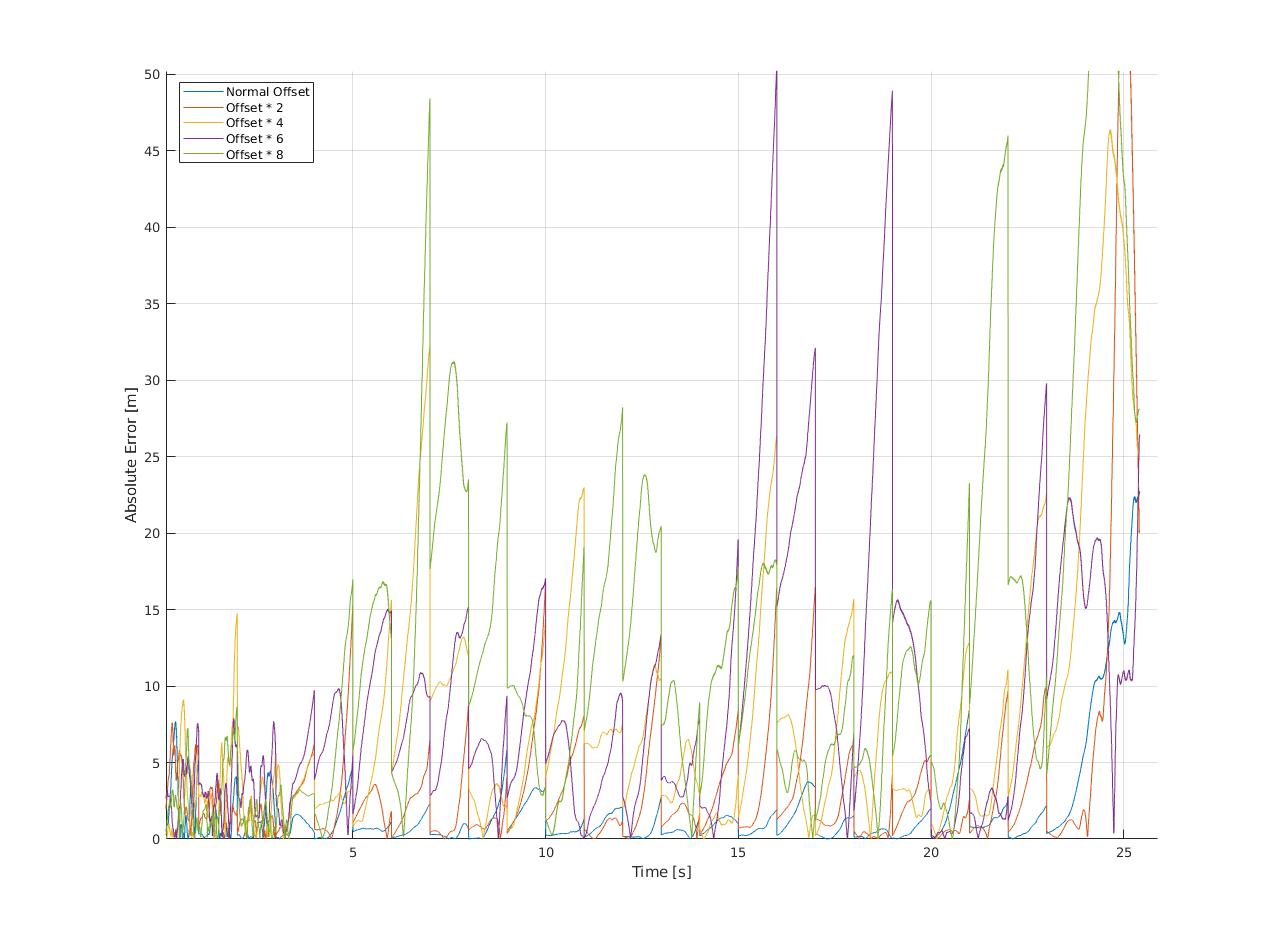
\includegraphics[width=0.8\textwidth]{./Pictures/PointMassOffsetErrorWithOffset.jpg}
 % PointMassOffsetErrorWithOffset.jpg: 0x0 pixel, 300dpi, 0.00x0.00 cm, bb=
  \caption{Error during flight time with different offsets}
 \label{fig:PointMassOffsetErrorWithOffset}
\end{figure}

\newpage
\section{Point Mass with Pressure}
As with the ones above the overall performance of the system model which uses the pressure as an additional state variable can be seen in Figure \ref{fig:PointMassPressurePerformance}.

\begin{figure}[h!]
 \centering
 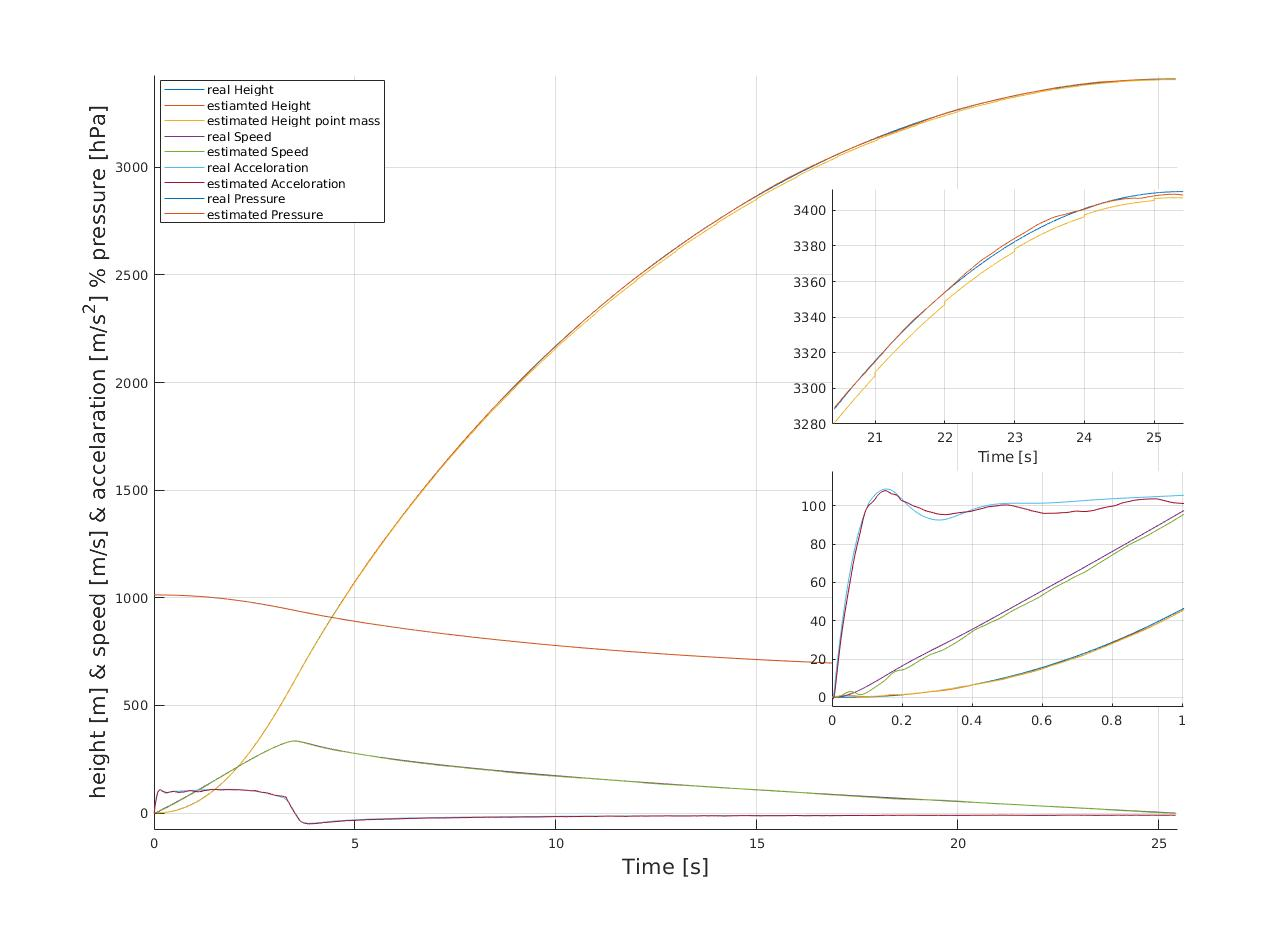
\includegraphics[width=.8 \textwidth]{./Pictures/PointMassPressurePerformance.jpg}
 % PointMassOffsetPerformance.jpg: 0x0 pixel, 300dpi, 0.00x0.00 cm, bb=
 \caption{Performance of point mass with pressure over time}
 \label{fig:PointMassPressurePerformance}
\end{figure}

This shows that it performs as good as a system which uses acceleration offset as a state value.
It can be seen that the pressure is so well estimated that it fully covers the real pressure curve in the plot.
Also in the plot of the first second it can be seen that there is no settling time for either of the estimation values.
The height in the last 5 second shows too that the impact from the GPS measurements are much smaller than in the first model (no staircase like adjustments of the height as seen in the point mass system model).

\begin{table}[h!]
\centering
\begin{tabular}{cccccc}
\hline
\multicolumn{1}{|c|}{State Variable} & \multicolumn{1}{c|}{Unit} & \multicolumn{1}{c|}{Max} & \multicolumn{1}{c|}{Min} & \multicolumn{1}{c|}{Mean} & \multicolumn{1}{c|}{Median} \\ \hline
Height                            & $m$                         & 5.16                   & 1.47e-06                 & 1.20                    & 0.96                      \\
Speed                             & $m/s$                       & 8.80                   & 0                        & 1.89                    & 1.61                      \\
Acceleration                      & $m/s^2$   			& 18.14                  & 3.90e-05                 & 1.80                    & 1.63                      \\
Pressure                  	  & $hPa$   			& 0.72                   & 4.69e-06                 & 0.13                    & 0.11
\end{tabular}
\caption{Error of estimated state variables point mass with pressure}
\label{tab:ErrorPointMassPressure}
\end{table}

Like above Table \ref{tab:ErrorPointMassPressure} shows the error over the simulations.
The error on the height is nearly as good as with the acceleration offset, while the maxima of the differences are quite smaller than above.
These results therefore have much better mean values of the errors.

\newpage
\subsection{Wrong Temperature Gradient}
While it does increase the accuracy it does also increase the needed computational effort due to the fact that to get a real added value from this,
the height out of the pressure has to be calculated at each time step with the help of the estimated pressure.
In addition when the temperature gradient is chosen wrong it deeply affects the estimation as can be seen in Figure \ref{fig:PointMassVSPressure}.
The errors there were low pass filtered with a moving average filter for better visualisation.

\begin{figure}[h!]
 \centering
 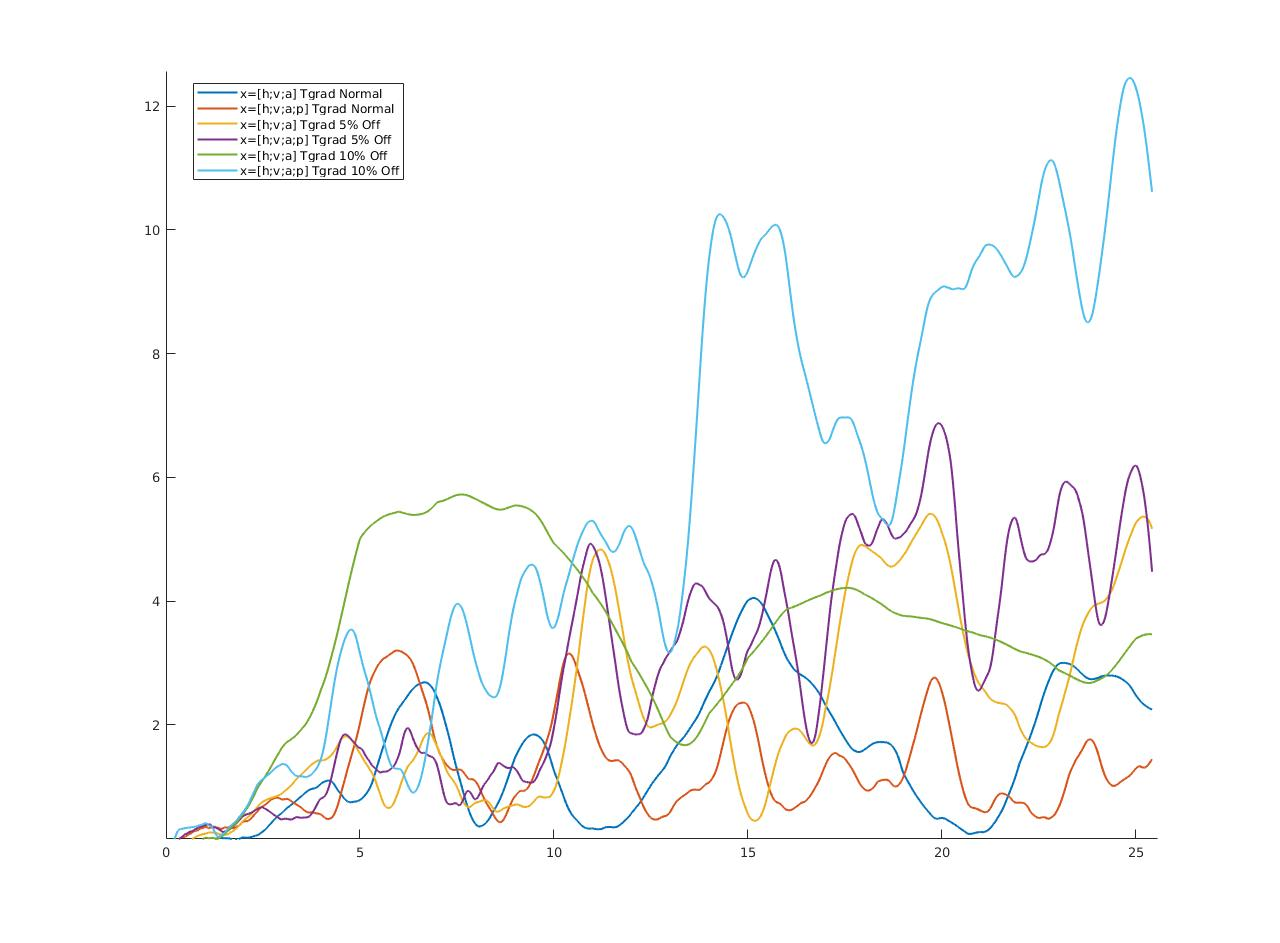
\includegraphics[width=.8 \textwidth]{./Pictures/PointMassVSPressure.jpg}
 % PointMassVSPressure.jpg: 0x0 pixel, 300dpi, 0.00x0.00 cm, bb=
 \caption{Plot of point mass vs the pressure low pass filtered}
 \label{fig:PointMassVSPressure}
\end{figure}

In this figure the error for both, a system with acceleration offset (which therefore can depend more on the accelerometer measurements)
and a system model with the pressure in the state vector are compared against each other.
While they preform equaly good as long as the temperature gradient is determined correctly,
if the gradient is determined wrong by just 5 percent it already performs less accurate than all of the other tested system models.
This is a problem due to the fact that the temperature gradient will most certainly not be correct during the whole flight.
With this it can be seen that the overall system performance of this model is more or less the same as with the normal point mass system.
On the other hand if the error on the temperature gradient is exactly known, the noise onto those measurements can be adjusted which
results in a gain of robustness for the whole estimation.

To summarize it, the pressure as a state variable is a risky but if done right a helpful adjustment of the system model.
\newpage
\section{Point Mass with Pitch Angle}
The pitch angle is difficult to estimate because it has no measured dependencies on its own.
Therefore the Kalman filter does just something like a real time low pass filtering on those measurements.
This can be seen in Figure \ref{fig:PointMassPitchAnglePerformance}. The estimated pitch angle there changes slower than the generated measurements value which can be seen in chapter \ref{ch:Implementation}.

\begin{figure}[h!]
 \centering
 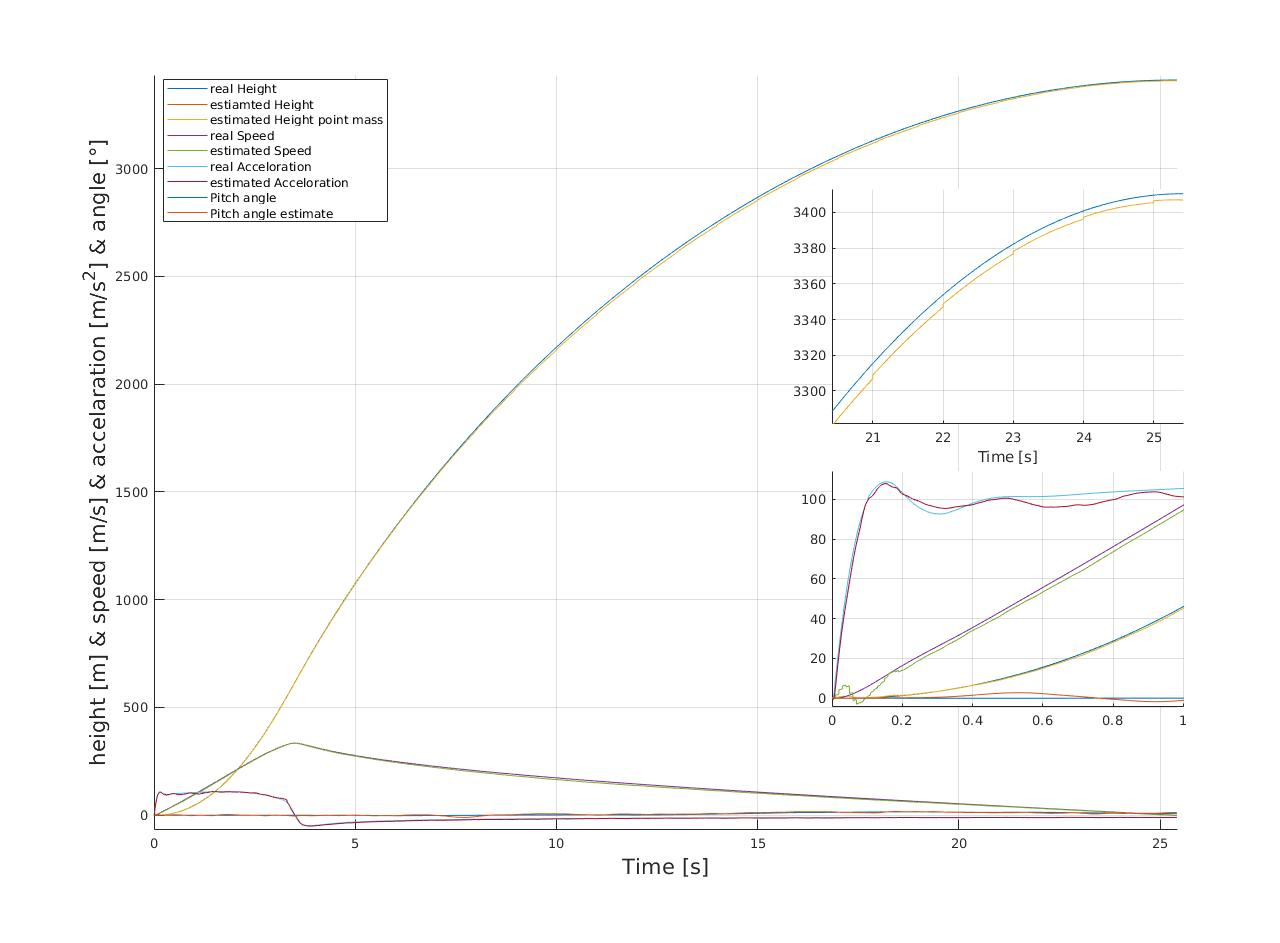
\includegraphics[width=.8 \textwidth]{./Pictures/PointMassPitchAnglePerformance.jpg}
 % PointMassOffsetPerformance.jpg: 0x0 pixel, 300dpi, 0.00x0.00 cm, bb=
 \caption{Performance of point mass with pitch angle over time}
 \label{fig:PointMassPitchAnglePerformance}
\end{figure}

The overall performance is more or less the same than that of the normal point mass system. This can espacially be seen in the last five seconds of the height estimation where both estimations are equal to each other (the estimation of the point mass system model does overlap the one of the system model which includes the pitch angle estimation).
The one big difference which can be seen in the plot of the first second is that the estimator tries to correct the wrong acceleration measurements (due to the offset) with the change of the pitch angle.
But because the system noise on the pitch angle states that it does not change in a great manner until the burnout the influence is restricted.

\begin{table}[h!]
\centering
\begin{tabular}{cccccc}
\hline
\multicolumn{1}{|c|}{State Variable} & \multicolumn{1}{c|}{Unit} & \multicolumn{1}{c|}{Max} & \multicolumn{1}{c|}{Min} & \multicolumn{1}{c|}{Mean} & \multicolumn{1}{c|}{Median} \\ \hline
Height                            & $m$                         & 20.24                  & 4.46e-06                 & 4.75                    & 2.24                      \\
Speed                             & $m/s$                       & 78.57                   & 0                        & 3.42                   & 2.44                      \\
Acceleration                      & $m/s^2$   			& 17.79                  & 6.26e-05                 & 1.68                    & 1.55                      \\
Angle	                  	  & $°$   			& 12.26                   & 2.46e-05                 & 2.41                  & 1.90
\end{tabular}
\caption{Error of estimated state variables point mass with pressure}
\label{tab:ErrorPointMassPitchAngle}
\end{table}

In Table \ref{tab:ErrorPointMassPitchAngle} the errors of the estimation can be seen once again.
It shows that the values are nearly the same as the ones from the point mass system.

\newpage
\subsection{Small Influence}
This results in the conclusion that the influence of the pitch angle is much smaller than thought.
This mainly because the pitch angle does only start to get to a greater value after the burnout.
After this the vertical acceleration is much smaller and therefore an error of the angle by a few degrees does not have a big impact.
In other words for example if the real angle is 10 degrees, the measurement at this point is around 18 degrees while the estimation is 11 degrees.
Then this means the measured acceleration of for example 10.15$m/s^2$ should be corrected to 10$m/s^2$. With the estimated angle it is corrected to 9.97$m/s^2$,
while with the measured angle it is corrected to 9.66$m/s^2$. So for this example an error of 8 degrees would only result in a false estimation of 0.31$m/s^2$.
Although this error does not develop in a linear fashion especially when the angle has a greater value, due to the rather small accelerations after the burnout the impact of the noisy measurements is still strongly limited.
This can be seen in the plot on Figure \ref{fig:PointMassVSPitch} where the estimation which uses the pitch angle as an additional state variable makes the performance just slightly better.
\begin{figure}[h!]
 \centering
 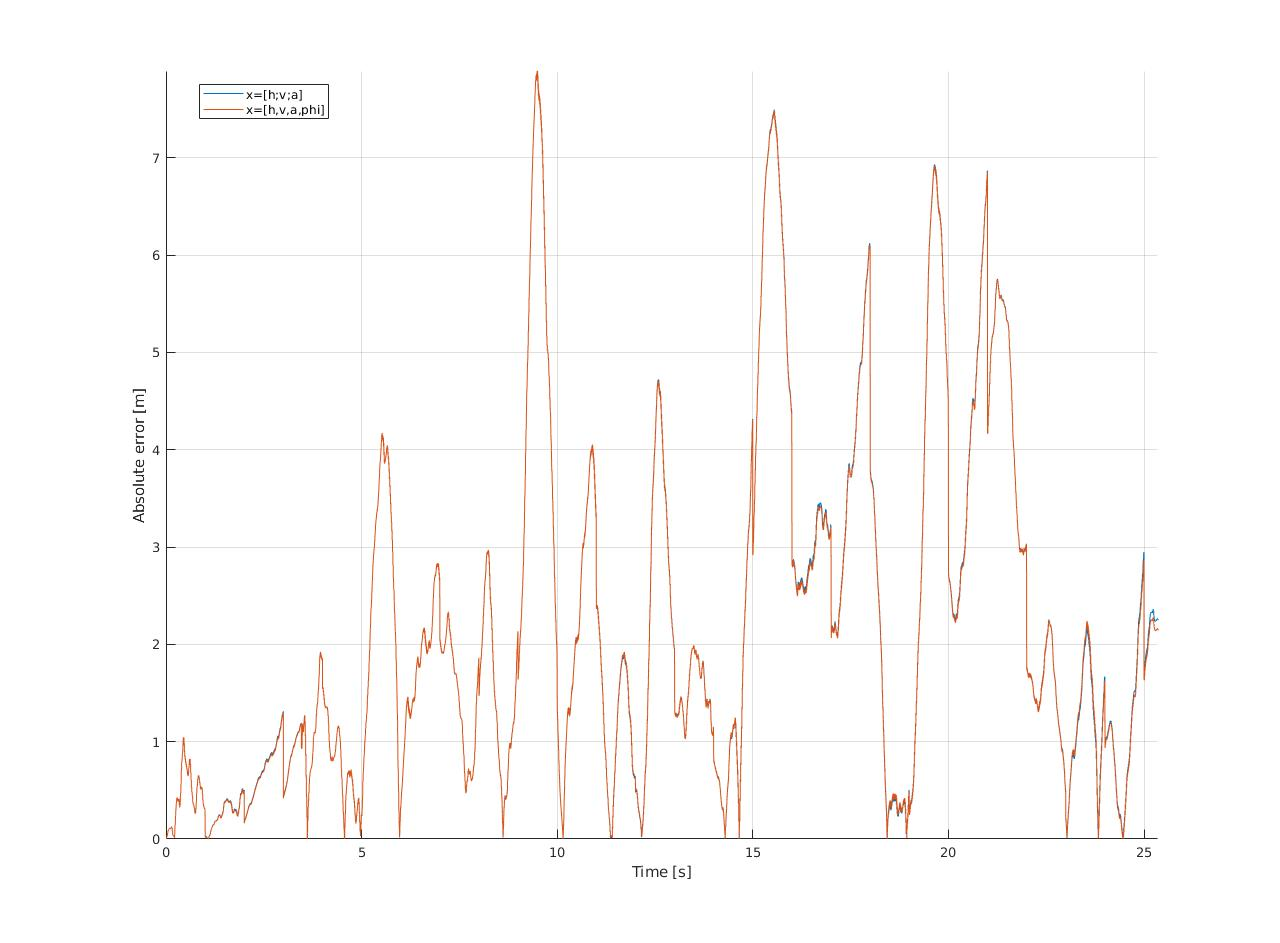
\includegraphics[width=.8 \textwidth]{./Pictures/PointMassVSPitch.jpg}
 % PointMassVSPitch.jpg: 0x0 pixel, 300dpi, 0.00x0.00 cm, bb=
 \caption{Estimation error over time from point mass system with and without pitch angle inclusion}
 \label{fig:PointMassVSPitch}
\end{figure}

\newpage
\section{Point Mass with Acceleration as Input}
The overall performance of this system model is shown in Figure \ref{fig:PointMassAccInputPerformance}.

\begin{figure}[h!]
 \centering
 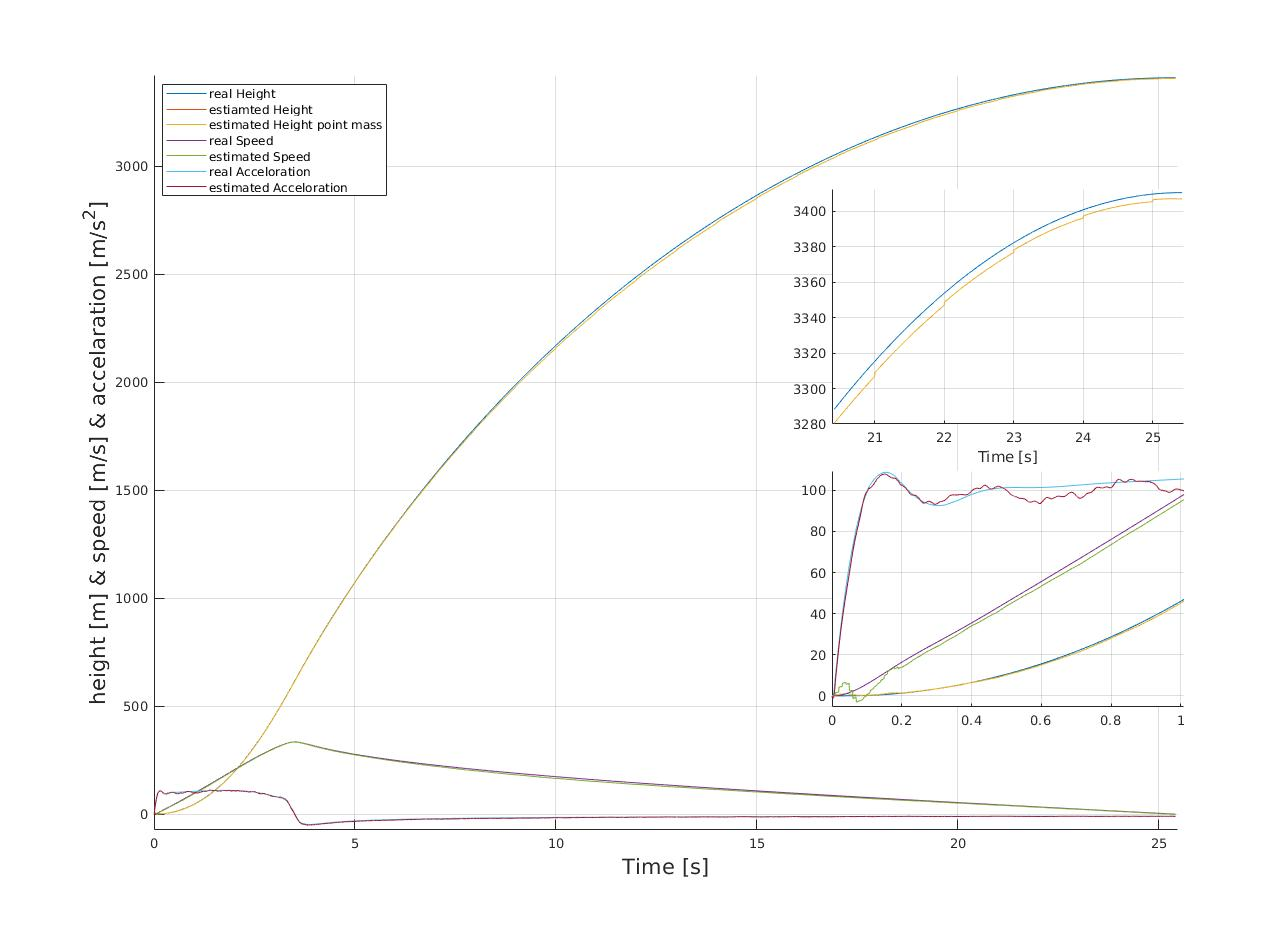
\includegraphics[width=.8 \textwidth]{./Pictures/PointMassAccInputPerformance.jpg}
 % PointMassOffsetPerformance.jpg: 0x0 pixel, 300dpi, 0.00x0.00 cm, bb=
 \caption{Performance of point mass with acceleration as input over time}
 \label{fig:PointMassAccInputPerformance}
\end{figure}

Its performance does also resemble the point mass system model quite well but without any significant improvement.
As above with the pitch angle the estimated height of both systems do overlap over more or less the whole flight.
This can be seen in the upper right corner of Figure \ref{fig:PointMassAccInputPerformance} where due to the overlap only the values from the point mass system model is visible.
The difference in the errors between this system model and the normal point mass model occurs more due to rounding errors of the simulation than due to really better estimation.
This can be concluded by fact that this system model performs sometimes slightly better and sometimes slightly worse than the point mass system, therefore there is no real gain in the implementation this way.

In addition the plot of the first second of the estimation shows that the acceleration estimation has more noise on it than in the other system models.
This is because the acceleration has no model dependencies in this implementation, it is taken directly as system input.
With this the system noise on the acceleration has to resemble either the measurement or the system noise.
In this implementation it was used to bring the measurement noise into the system and therefore the low pass characteristics of the system noise is lost.
In other words with a measurement as input a tuning parameter (either system or measurement noise) which could compensate the corresponding state value cannot be used.
So there is no real gain in this implementation and it will therefore not be implemented in the final system model.

\begin{table}[h!]
\centering
\begin{tabular}{cccccc}
\hline
\multicolumn{1}{|c|}{State Variable} & \multicolumn{1}{c|}{Unit} & \multicolumn{1}{c|}{Max} & \multicolumn{1}{c|}{Min} & \multicolumn{1}{c|}{Mean} & \multicolumn{1}{c|}{Median} \\ \hline
Height                            & $m$                         & 20.05                  & 7.21e-06                 & 4.71                    & 2.18                      \\
Speed                             & $m/s$                       & 78.49                  & 0                        & 3.38                    & 2.40                      \\
Acceleration                       & $m/s^2$   			& 10.65                  & 0                        & 1.60                    & 1.43
\end{tabular}
\caption{Error of estimated state variables point mass with acceleration as input}
\label{tab:ErrorPointMassAccelerationInput}
\end{table}

\newpage
\section{Point Mass with Offset and Better Calculated System Noise}
The better calculated system noise for this estimation was calculated as stated in chapter \ref{ch:Implementation}.
This has been done by calculating the discrete system noise matrix Gd with the integration method as well as
derive the perfect measurements and then low pass filter them to get better system noise vectors.
This improvement had to be done on a system which uses the acceleration offset as well in the state vector to get the maximum possible gain out of this implementation.
This results in an overall system performance as seen in Figure \ref{fig:PointMassBetterNoisePerformance}

\begin{figure}[h!]
 \centering
 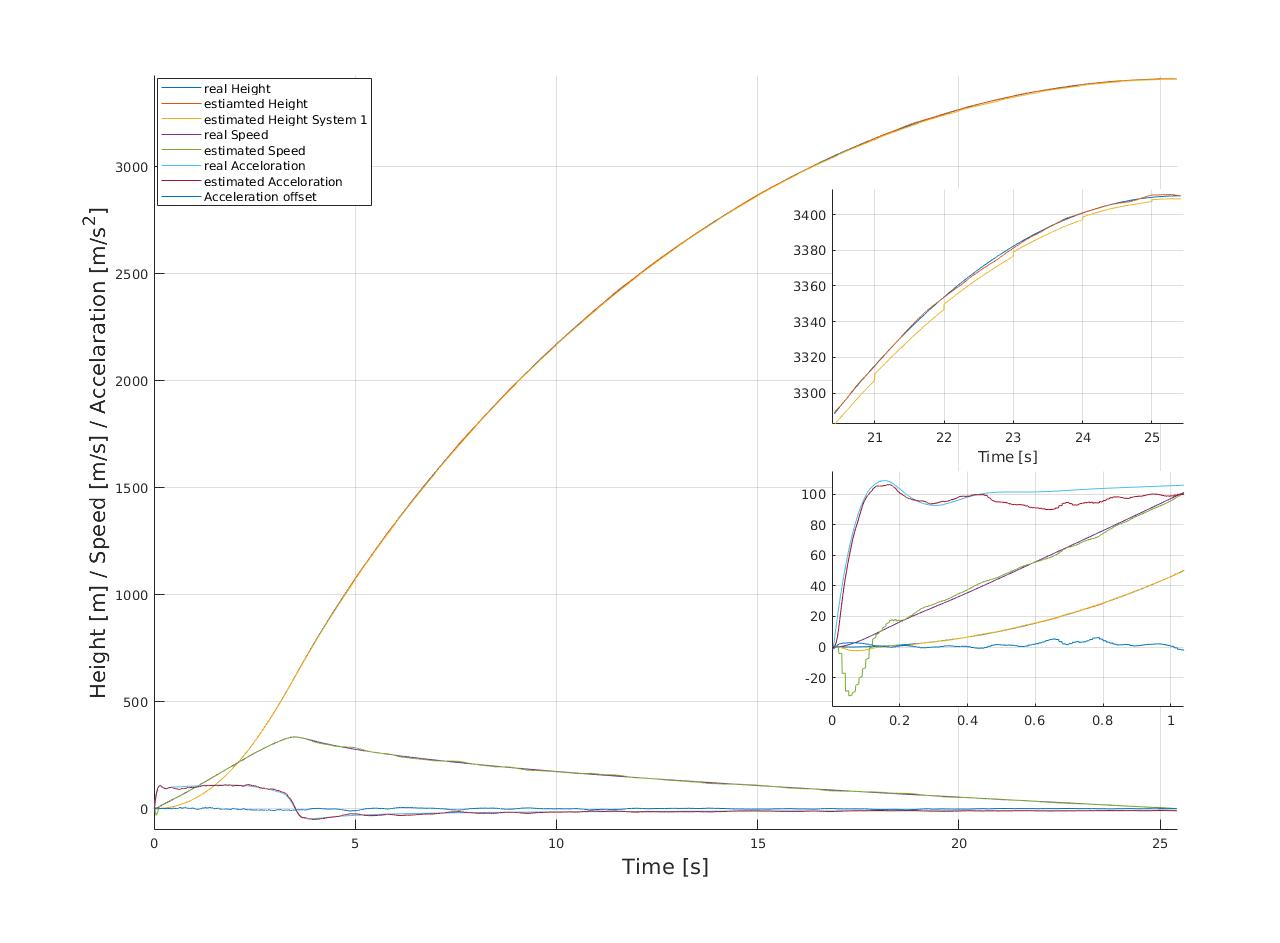
\includegraphics[width=.8 \textwidth]{./Pictures/PointMassBetterNoisePerformance.jpg}
 % PointMassOffsetPerformance.jpg: 0x0 pixel, 300dpi, 0.00x0.00 cm, bb=
 \caption{Performance of point mass with better system noise over time}
 \label{fig:PointMassBetterNoisePerformance}
\end{figure}

This system performs much like the one with acceleration offset as a state vector.
The greatest difference can be seen in the first half second where the acceleration is nearly perfectly estimated.
Also does the acceleration offset not change as much as in the system model without the improved system noise calculation.
This is because with the better system noise an optimal estimation can be achieved with less effort since the influence of the acceleration offset is more clearly defined.

\begin{table}[h!]
\centering
\begin{tabular}{cccccc}
\hline
\multicolumn{1}{|c|}{State Variable} & \multicolumn{1}{c|}{Unit} & \multicolumn{1}{c|}{Max} & \multicolumn{1}{c|}{Min} & \multicolumn{1}{c|}{Mean} & \multicolumn{1}{c|}{Median} \\ \hline
Height                            & $m$                         & 9.74	                  & 8.11e-06                 & 1.28                    & 0.73                      \\
Speed                             & $m/s$                       & 78.58                   & 0                        & 2.79                    & 1.85                      \\
Acceleration                       & $m/s^2$   			& 86.93                   & 4.07e-05                 & 3.57                    & 1.96                     \\
Acceleration Offset                & $m/s^2$   			& 88.60                   & 2.52e-05                 & 4.59                    & 2.59
\end{tabular}
\caption{Error of estimated state variables point mass with acceleration offset and better system noise}
\label{tab:ErrorPointMassBetterNoise}
\end{table}

Table \ref{tab:ErrorPointMassBetterNoise} shows that the system performs pure error wise better than each of the other system models discussed before.
While it also contains big maxima in speed, the acceleration and acceleration offset values are smaller than the ones of the system with only acceleration offset.
Due to that the mean values (except the offset) are still better than most other.

Figure \ref{fig:PointMassVSBetterNoise} shows that an overall better estimation can be achieved with this tactic.
\begin{figure}[h!]
 \centering
 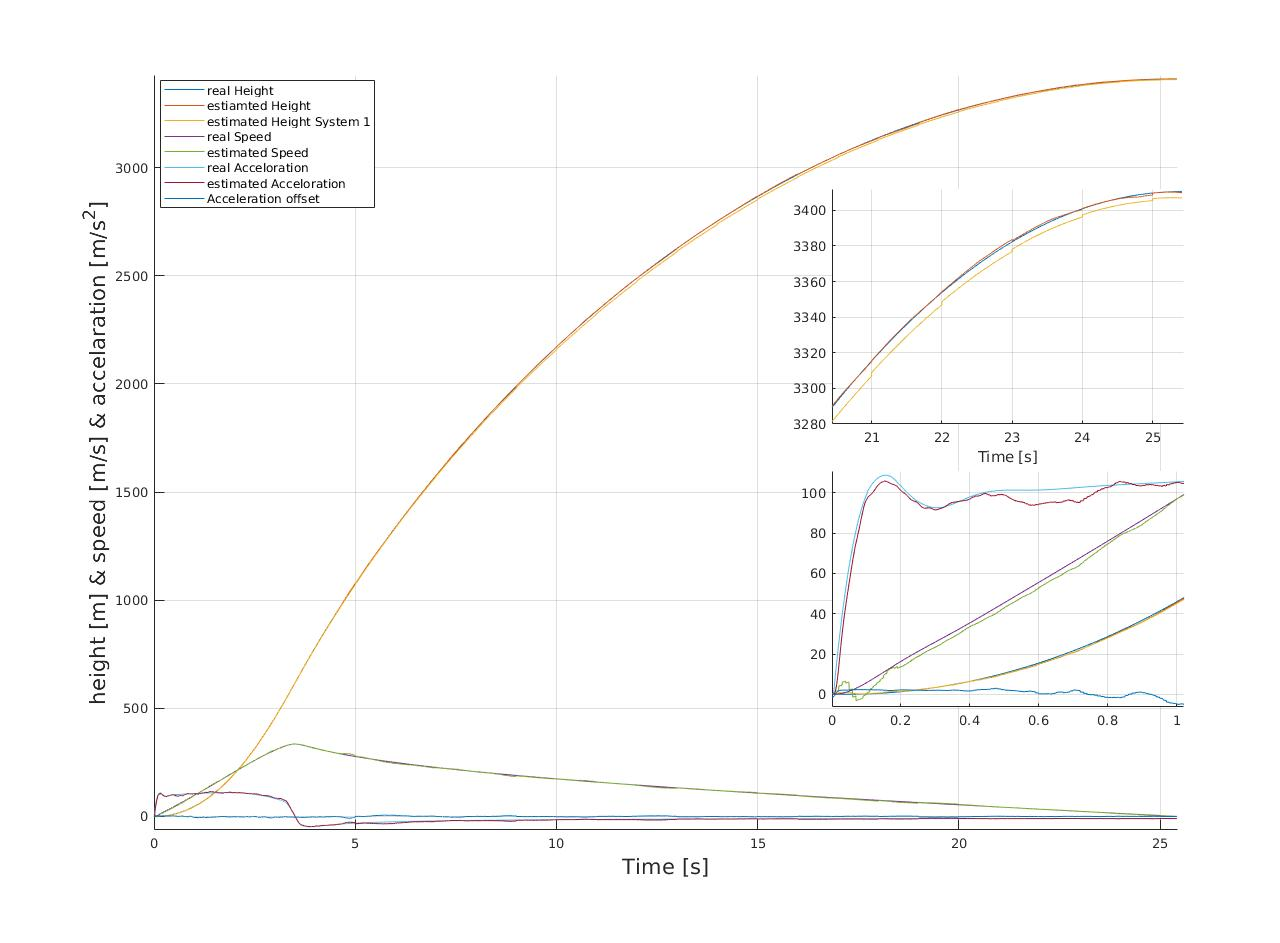
\includegraphics[width=.8\textwidth]{./Pictures/PointMassVSBetterNoise.jpg}
 % PointMassVSBetterNoise.jpg: 0x0 pixel, 300dpi, 0.00x0.00 cm, bb=
 \caption{Error over time with and without better system noise}
 \label{fig:PointMassVSBetterNoise}
\end{figure}
This is mostly due to the better system noise vector which can be much better estimated this way.
Also the additional effort to access this system model only occurs on the preparation,
while it does have no effect on the computational effort during the flight itself.
So this approach of the state estimation should be used any time if available.

\section{With and Without GPS}
It is not certain that the GPS will be working in the next competitions as already stated in the introduction.
In addition the GPS sensor data needs more time to be measured and can therefore arrive too late to be included correctly.
There is the possibility of back calculation to include such too late arrived measurements into the state estimation but this needs a lot of computational effort \cite{SimonDan2006Ose:}.

Because of this, the estimation without the GPS measurements are tested with a point mass system model to find its direct impacts.
Figure \ref{fig:PointMassWithWithoutGPS} shows the plot of different estimations with and without working GPS.

\begin{figure}[h!]
 \centering
 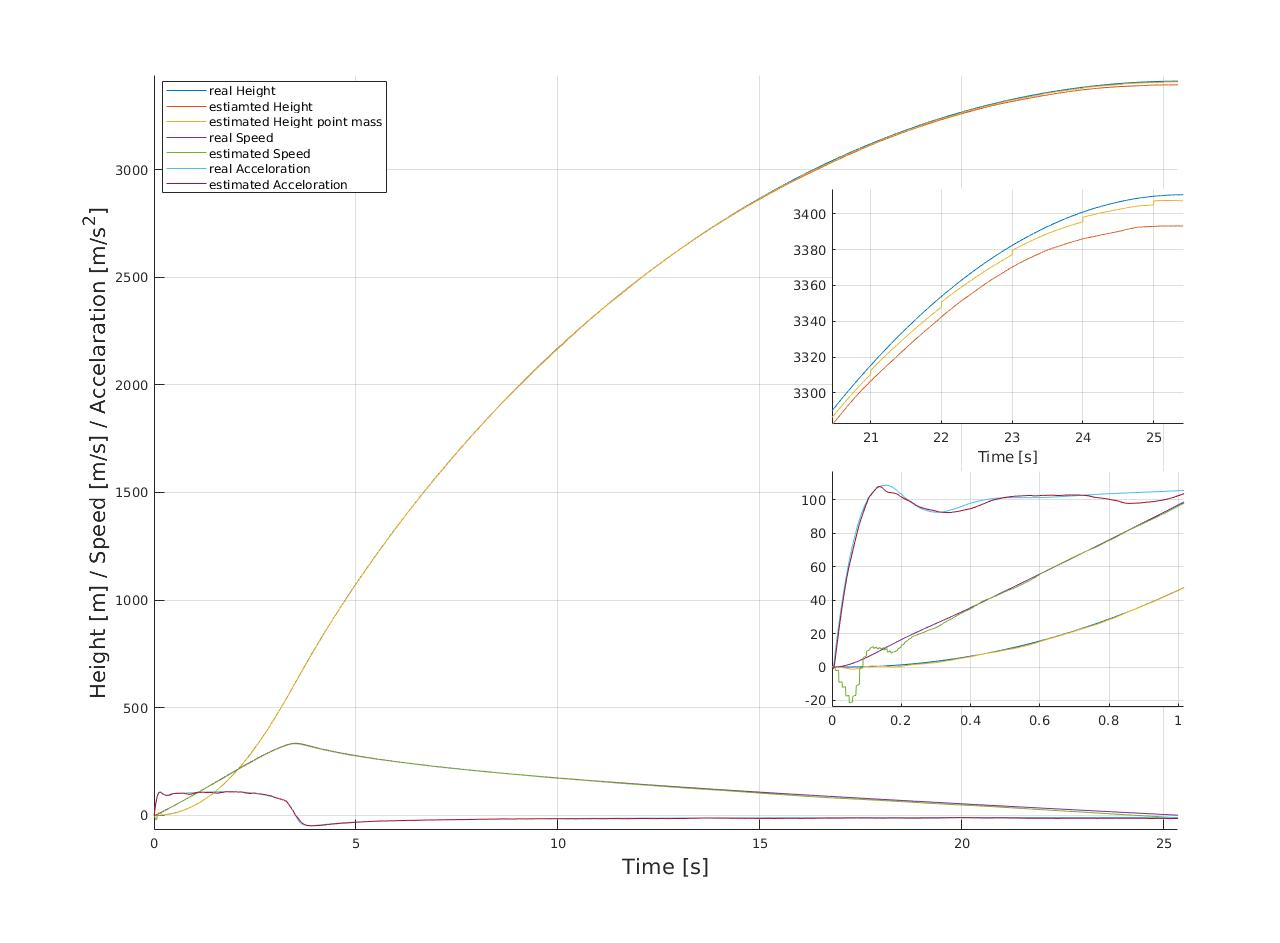
\includegraphics[width=.8 \textwidth]{./Pictures/PointMassWihtoutGPSPerformance.jpg}
 % PointMassOffsetPerformance.jpg: 0x0 pixel, 300dpi, 0.00x0.00 cm, bb=
 \caption{Performance of point mass without GPS over time}
 \label{fig:PointMassWithoutGPSPerformance}
\end{figure}

As expected the height is further away from the ground truth in the last five seconds plot than the one estimated with GPS measurements.
Also the staircase like correction steps which come from the GPS measurements are missing.
This behaviour was expected because the the GPS measurements are most important at great heights were the remaining measurements lose their credibility.


\begin{table}[h!]
\centering
\begin{tabular}{cccccc}
\hline
\multicolumn{1}{|c|}{State Variable} & \multicolumn{1}{c|}{Unit} & \multicolumn{1}{c|}{Max} & \multicolumn{1}{c|}{Min} & \multicolumn{1}{c|}{Mean} & \multicolumn{1}{c|}{Median} \\ \hline
Height                            & $m$                         & 31.20                  & 5.77e-05                 & 8.97                    & 5.20                      \\
Speed                             & $m/s$                       & 78.58                  & 0                        & 6.35                    & 4.86                      \\
Acceleration                       & $m/s^2$   			& 17.78                  & 7.60e-05                 & 3.48                    & 2.34
\end{tabular}
\caption{Error of estimated state variables point mass without GPS measurements}
\label{tab:ErrorPointMassWithoutGPS}
\end{table}

Table \ref{tab:ErrorPointMassWithoutGPS} which displays the errors from the estimations shows that as expected the error is bigger in each value.
Also the maximum height error of over 30 meter shows that the normal state estimator is really depending on the GPS measurements.

\newpage
\subsection{Wrong Temperature Gradient}
This system has to depend strongly on the barometer measurements to calculate the height.
Therefore the problem of a wrong temperature gradient arises once again.
To show this the estimation results with different temperature gradients are plotted in Figure \ref{fig:PointMassWithWithoutGPS}.

\begin{figure}[h!]
 \centering
 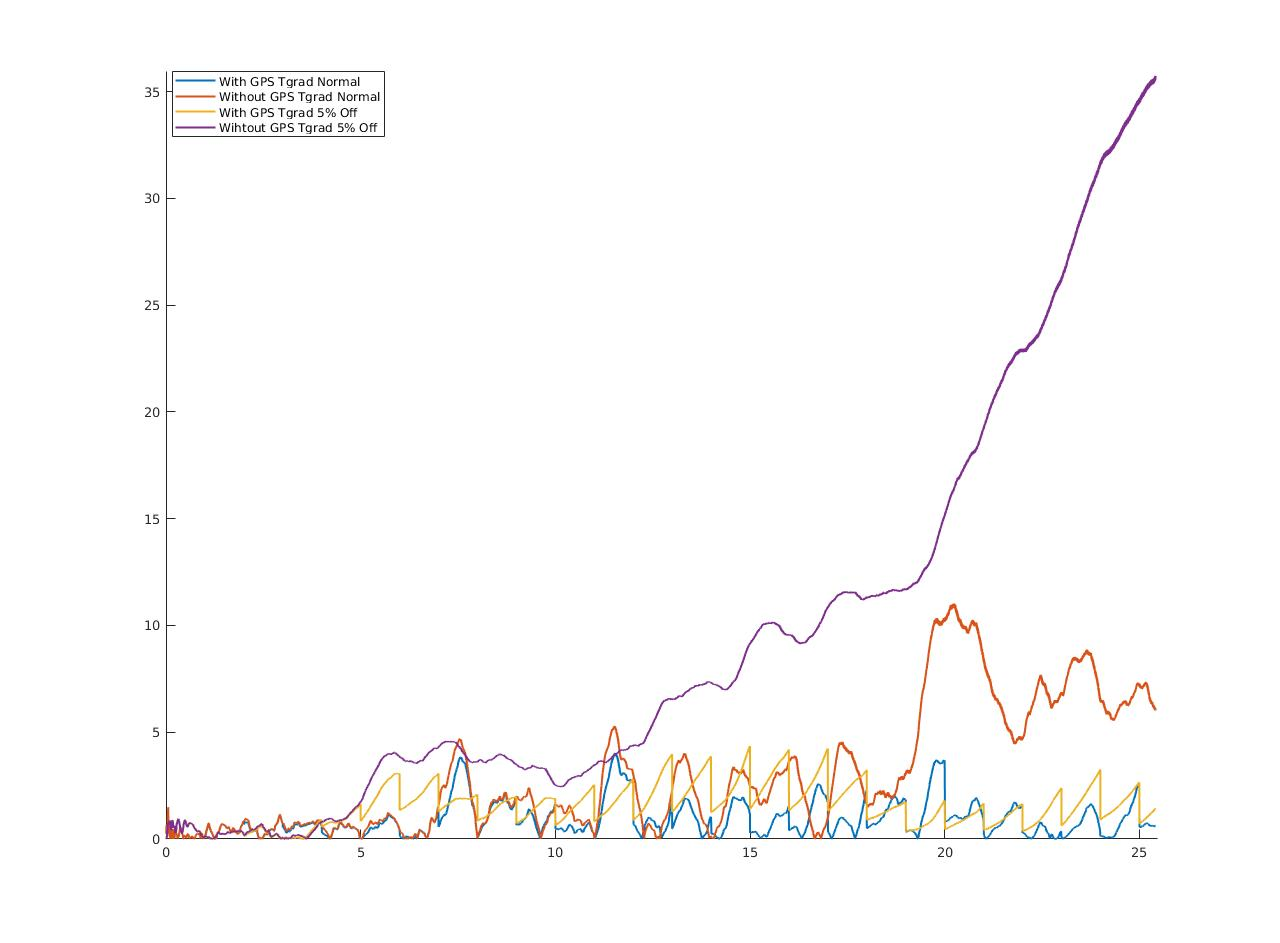
\includegraphics[width=.8\textwidth]{./Pictures/PointMassWithWithoutGPS.jpg}
 % PointMassWithWithoutGPS.jpg: 0x0 pixel, 300dpi, 0.00x0.00 cm, bb=
 \caption{Absloute error over time with and without GPS}
 \label{fig:PointMassWithWithoutGPS}
\end{figure}

It shows that especially if the temperature gradient is chosen wrong (by just 5 percent) and
therefore the height out of the pressure measurements is calculated wrong the error of the estimation rises significantly.
With this the error increases with the ascending rocket if it is not corrected by the GPS measurements.
So the aim of the best performance system has to be that it should not depend too much on those GPS measurements for a good state estimation.

\section{Best Performing System}
Based on the results from the tests above the best performing system can be defined.
The main goal is to achieve an as robust state estimation as possible that does also match the given accuracy requirements.
The pitch angle did not have a useful positive effect on the estimation and would increase the computational effort due an additional rank, because of this it is not implemented.
Also the acceleration as input does not significantly improve the estimation.
Therefore the best system for the stated problem consist of the additional acceleration offset as a state vector as well as better calculated system noise.
Despite the fact that the pressure is risky to implement as a state variable it is used in this implementation because it does increase the robustness significantly.
This does therefore result in a rank 5 system which should fit the given calculation steps requirement at first glance, but it will also be analyzed in detail in the next chapter.

\begin{figure}[h!]
 \centering
 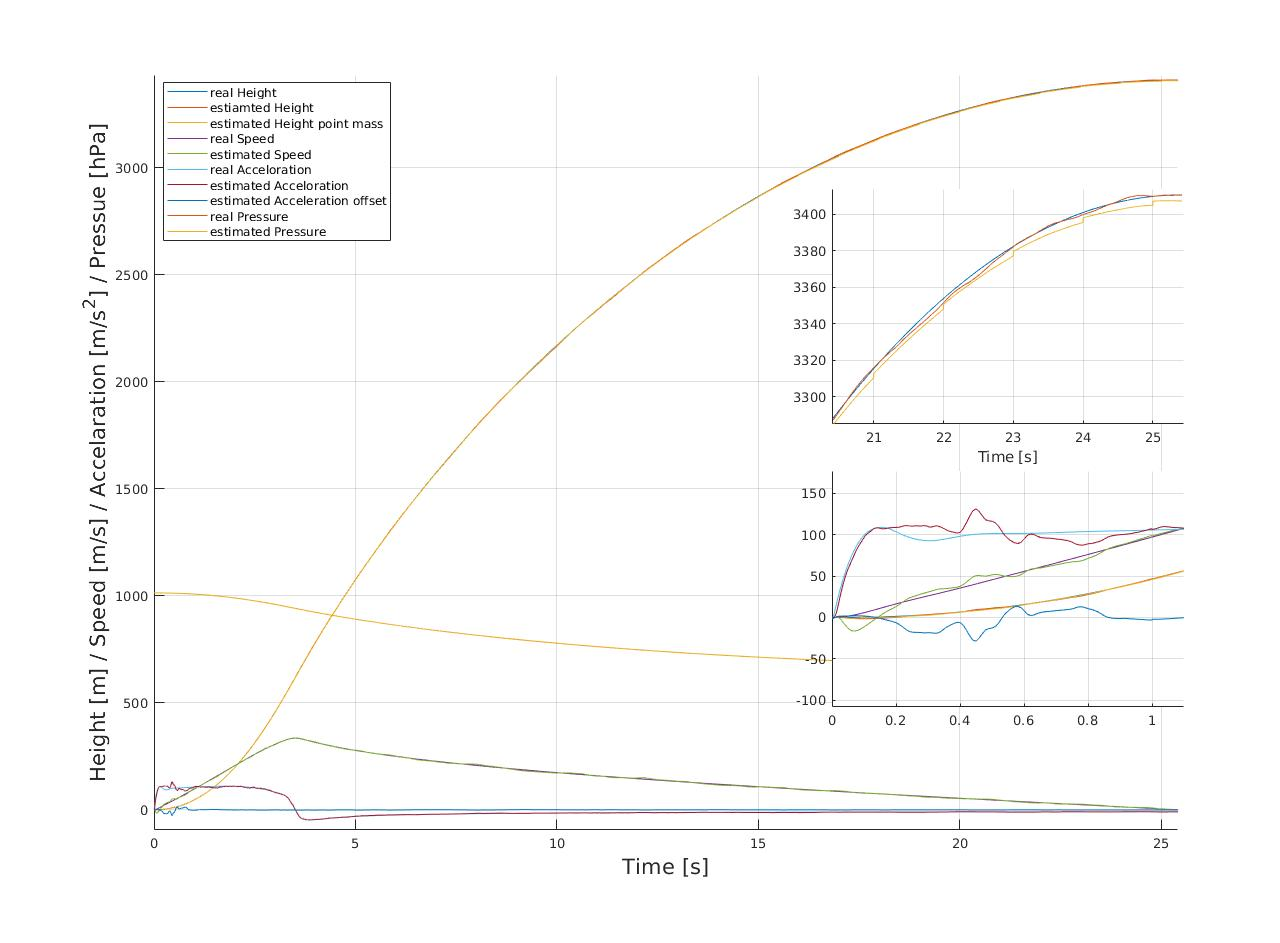
\includegraphics[width=.8\textwidth]{./Pictures/BestSystemPerformance.jpg}
 % BestSystemPerformance.jpg: 0x0 pixel, 300dpi, 0.00x0.00 cm, bb=
 \caption{Performance over time}
 \label{fig:BestSystemPerformance}
\end{figure}

Figure \ref{fig:BestSystemPerformance} shows again the performance over one whole flight.
In the plot in the lower right corner which shows the first second of the estimation it can be seen that this system has a clearly visible settling time in the acceleration and speed.
While this seems quite big at the first sight, it is well in the given requirements of one second settling time after the burnout.
On the other hand it shows that the performance increases significantly after the acceleration and speed have settled.
This increase in the accuracy of the estimation can also be seen in the table \ref{tab:ErrorBestPerformanceSystem}.

\begin{table}[h!]
\centering
\begin{tabular}{cccccc}
\hline
\multicolumn{1}{|c|}{State Variable} & \multicolumn{1}{c|}{Unit} & \multicolumn{1}{c|}{Max} & \multicolumn{1}{c|}{Min} & \multicolumn{1}{c|}{Mean} & \multicolumn{1}{c|}{Median} \\ \hline
Height                            & $m$                         & 7.39	                  & 2.01e-06                 & 1.26                    & 0.92                      \\
Speed                             & $m/s$                       & 24.87                   & 0                        & 1.61                    & 1.26                      \\
Acceleration                       & $m/s^2$   			& 41.66                   & 4.86-06                  & 1.28                    & 0.70                     \\
Acceleration Offset                & $m/s^2$   			& 41.70                   & 5.36e-06                 & 1.01                    & 0.61                     \\
Pressure		          & $hPa$   			& 0.80                    & 2.49e-06                 & 0.14                    & 0.12
\end{tabular}
\caption{Error of estimated state variables of the best found system}
\label{tab:ErrorBestPerformanceSystem}
\end{table}

While the median of the error from the estimated height shows a slight loose in the height accuracy in comparison to the system model with better system noise alone,
the accuracy of all other values has increased.
This is especially impressive in the mean of the speed and acceleration, because they have big errors at the beginning with the shown settling problem which has been shown in the plot above.
Also the height is with a median of just 0.82 meter and a maximum of 7.39 meter still most of the time in the aimed error of 2 meter maximal error.

\subsection{Robustness}
The slight loss in accuracy was traded for an increase in robustness which is seen as more important due to different uncertainties,
which are still being able to function properly if a sensor fails as well as being robust against wrong system modelling
and especially falsely detected temperature gradients. The impact of those possible errors on the found best performing system will be shown in the following sections.

\subsubsection{Without GPS}
As stated above this system should estimate the height without a significant raise in the error without the GPS measurements.
Figure \ref{fig:ErrorWitoutGPS} shows the height error of the best performing system model without GPS measurements.
For comparison there is also the point mass system model estimation with and without the GPS measurements plotted.

\begin{figure}[h!]
 \centering
 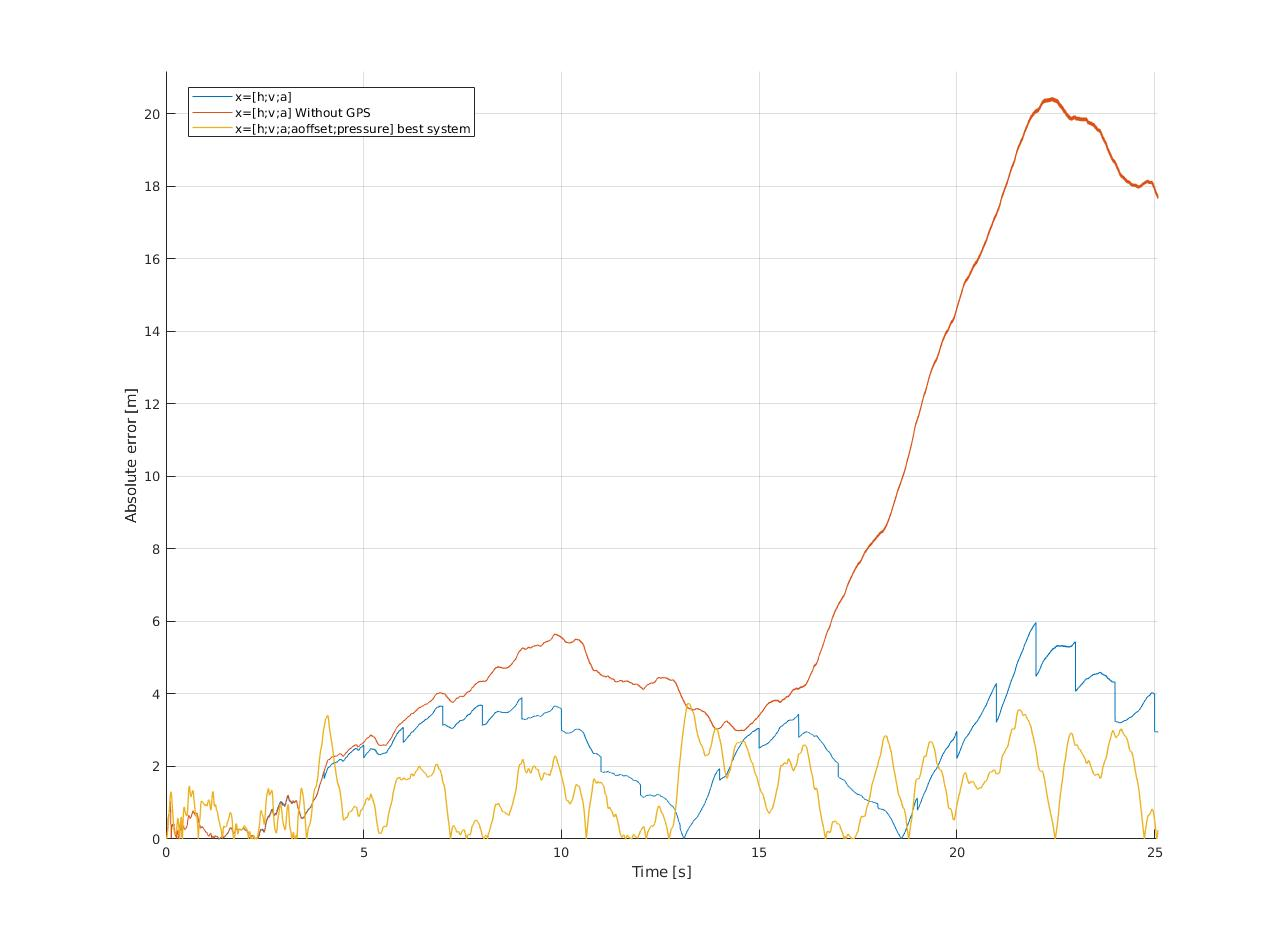
\includegraphics[width=.8\textwidth]{./Pictures/ErrorPointMassBestSystemWithoutGPS.jpg}
 % ErrorPointMassBestSystemWithoutGPS.jpg: 0x0 pixel, 300dpi, 0.00x0.00 cm, bb=
 \caption{Error of point mass system and best system with and without GPS measuements}
 \label{fig:ErrorWitoutGPS}
\end{figure}

This shows that the best found system model can estimate the height as good as the point mass system without the GPS measurements.
On the other hand the point mass system model without the GPS measurements does loose accuracy as the rocket rises higher above ground.

\subsubsection{Wrong Temperature Gradient}
This system model should also have some robustness against a falsely defined temperature gradient.
It has to be said that in the simulation the difference of the real and the used temperature gradient is known and the noises are adjusted properly.
This will maybe not be the case in the real flight.
Table \ref{tab:ErrorChangingTempGradWithWithoutGPS} shows the errors which the state estimation makes when the temperature gradient is wrong with and without working GPS.

\begin{table}[h!]
\centering
\begin{tabular}{ccc}
\hline
\multicolumn{1}{|c|}{Temperature gradient correctness} & \multicolumn{1}{|c|}{Mean}& \multicolumn{1}{|c|}{Median} \\ \hline
Normal with GPS 	& 1.26 		& 0.92\\
Normal without GPS	& 1.43	 	& 1.11\\
5\% off with GPS 	& 2.77	 	& 2.46\\
5\% off without GPS 	& 3.39	 	& 3.24\\
10\% off with GPS 	& 6.32	 	& 7.04\\
10\% off without GPS 	& 7.74 		& 7.61
\end{tabular}
\caption{Error of the height in meter by changing temperature gradient with and without GPS measurements}
\label{tab:ErrorChangingTempGradWithWithoutGPS}
\end{table}

First of all it can be seen that with the correct temperature gradient and no GPS measurements,
the error of the height estimation is still clearly below the two meter margin.
In addition the median of the height error does only increases by around one meter if no GPS is available.
But also the robustness of this system model can be seen, if there are no GPS measurements
and the temperature gradient is 10 percent off over the whole flight it only results in a median error of the height estimation of 7.61 meter.

\section{Sensor Outfall}
In addition to the tests for the different system model implementation
the possibility to simulate outfalls of the different sensors at start or during the flight was implemented for the last system model.
For this the corresponding measurement noise of this sensor values can be set to infinity at a given time step.
The most probable way was found that a sensor fails during the burning of the motor because of to the vibrations.
Therefore the here discussed scenarios are all the same with the corresponding sensor failing at the third second of the flight while the motor is still burning.

\subsection{GPS Outfall}
The outfall of the GPS has already been discussed above for a state estimation with no GPS measurements at all.
If the GPS fails during the flight the behaviour of the state estimation should resemble the one above after the outfall.
The tests have shown that this is the case.
If the GPS fails at second three the mean of the height error rises to 1.42 meter while the median rises to 1.11 meter.
The other state variable errors rise by a small amount too, but as expected the pressure estimation error stays the same.
These values show that the estimation is just slightly better than without any GPS at all.

\subsection{Barometer Outfall}
The barometer is special because if all barometers are lost,
the height which is calculated out of the state vector pressure has to be completely max'ed out.

\subsubsection{One Barometer Fails}
The loss of one barometer does already make a significant change into the estimation.
For example the mean of the height error rises to 1.78 meter while the median also rises to 1.39 meter.
The difference between the mean and the median shows that there occur more outliers if just one barometer is active.
This can also be seen in the error of the barometer estimation which rises to 0.2 hP for the mean and 0.16 hP for the median.

\subsubsection{All Barometer Fail}
More interesting is how the state estimator is performing when no barometer measurements are available at all.
As expected the error of the barometer estimation rises to high values which are around 12 hP for the mean and 11 hP for the median.
But on the other hand the accuracy of the height estimation does actually rise to more or less the same values as with two working barometers.
This behaviour can be explained with the still working GPS.
If both barometers fall out and therefore there is no height calculated out of the pressure, the height from the
GPS sensor gets a higher weight due to it being the only remaining measurements on the height.
\newpage
\subsection{Accelerometer Outfall}
The influence of an outfall of the accelerometer can be well shown in the plots of Figure \ref{fig:PerformanceAccOutfall}.

\begin{figure}[h!]
 \centering
 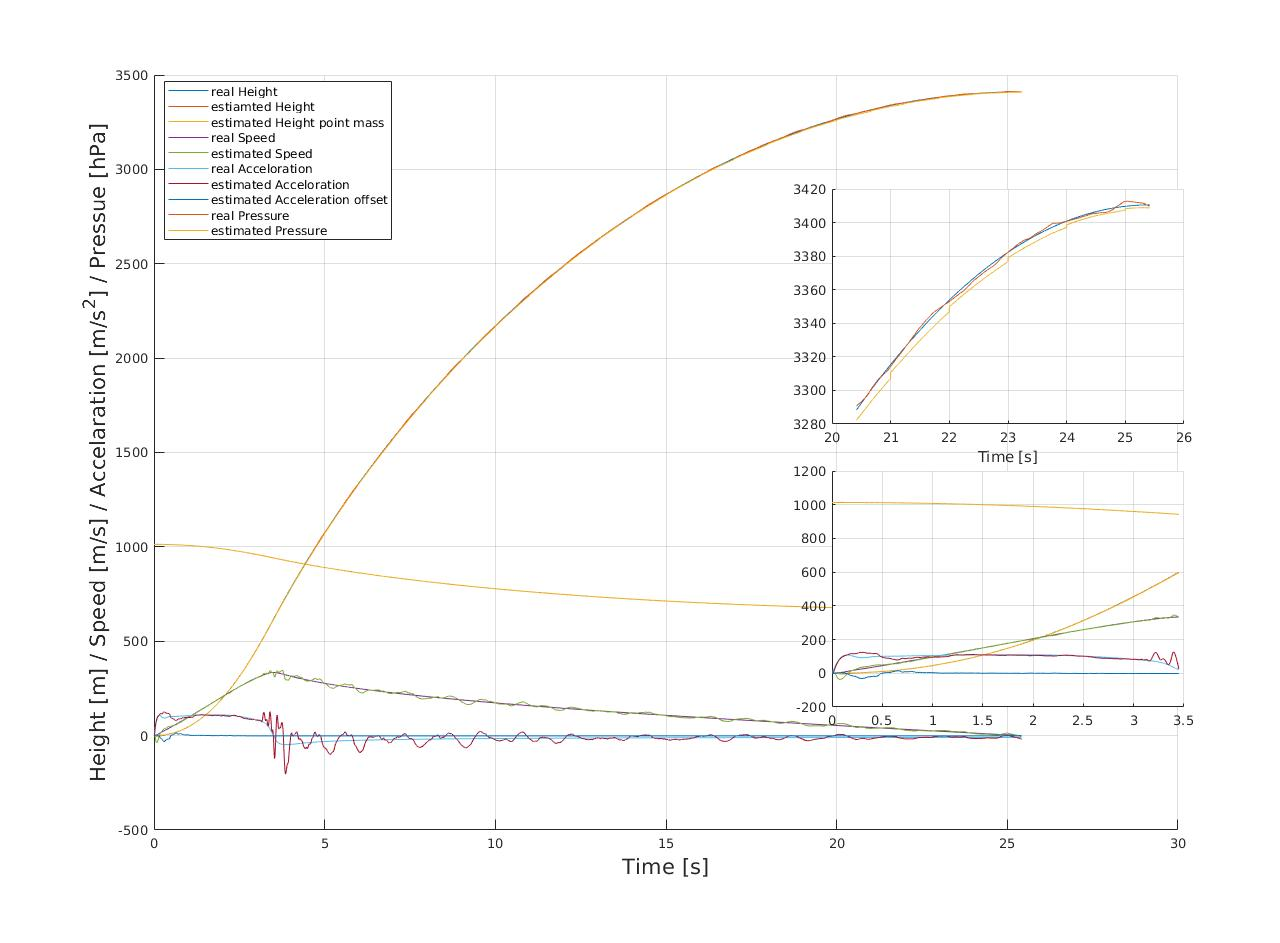
\includegraphics[width=.8\textwidth]{./Pictures/BestSystemPerformanceAccOutfall.jpg}
 % ErrorPointMassBestSystemWithoutGPS.jpg: 0x0 pixel, 300dpi, 0.00x0.00 cm, bb=
 \caption{Performance over a whole flight with failing accelerometer at second 3}
 \label{fig:PerformanceAccOutfall}
\end{figure}

It shows how the acceleration estimation starts to change in a great manner after the third second.
But as can be seen in the plot of the last five seconds the height estimation does not change in a great manner
compared to the estimation with acceleration measurements during the whole flight.
The calculated height errors do confirm this by values of 1.54 meter for the mean and 1.20 meter for the median.
The pressure estimation is also not impacted as it was expected it would be.
On the other hand the error of the acceleration does rise by around 10 $m/s^2$ and does therefore affect the speed estimation.

\subsection{Gyrometer Outfall}
Due to the fact that the pitch angle does not have such a big impact onto the acceleration as already stated above,
the effect onto the state estimation if the gyrometer fails is also quite small.
First of all the error which is made in the estimation of the acceleration should be examined.
Against the expectation it does rise by around 1$m/s^1$ for both the mean and the median value.
Due to that the estimation of the height does also loose some accuracy and resembles with 1.39 meter for the mean
and 1.11 meter for the median the same situation as if there would be no GPS measurements.
This shows that while it is not necessary to estimate the pitch angle the measurements of the gyrometer should still be included for an optimal estimation.

\newpage
\subsection{Multiple Sensor Outfall}
A requirement which has been given is that the sensor fusion should still be able to work with 2-3 sensors failing.
Two sensors was already discussed by tailking about both barometer or the accelerometer
(which would also be an outfall of the gyrometer, since those measurements would not be included either) failing.
An additional test should therefore be on what happens when three sensors fail.
For this scenario the two barometers and the gyrometer were chosen to fail because if they fail the observability of the point mass system still remains.

\begin{figure}[h!]
 \centering
 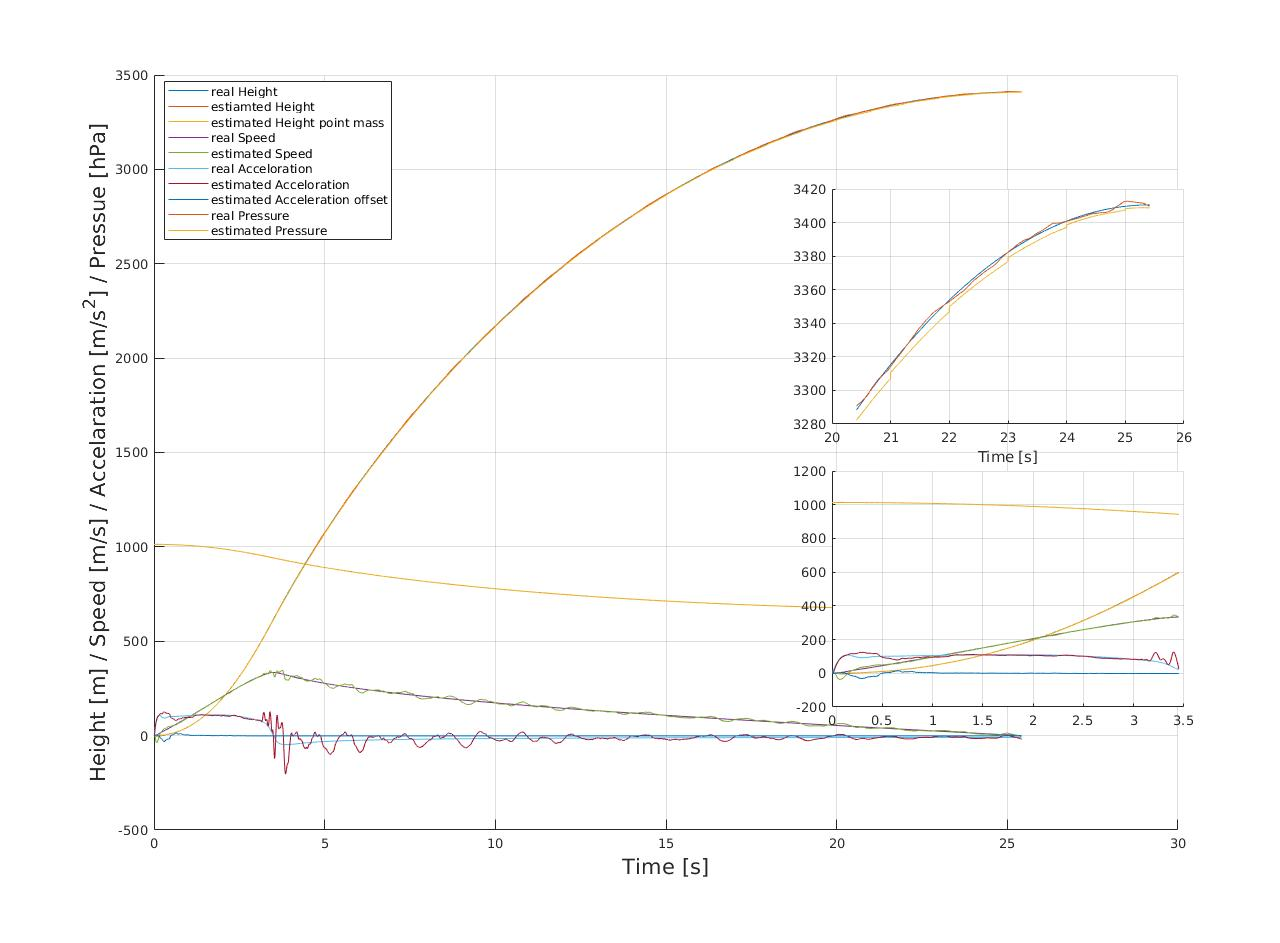
\includegraphics[width=.8\textwidth]{./Pictures/BestSystemPerformanceAccOutfall.jpg}
 % ErrorPointMassBestSystemWithoutGPS.jpg: 0x0 pixel, 300dpi, 0.00x0.00 cm, bb=
 \caption{Performance over a whole flight with both barometer and the gyrometer failed}
 \label{fig:PerformanceMOutfall}
\end{figure}

With those failed sensors the estimation does still work quite well which can be seen in the plots of Figure \ref{fig:PerformanceMOutfall}.
This is because the GPS which provides the most accurate measurements is still working.
Due to that the error of the height estimation does just rise slightly to 1.54 meter for the mean and 0.97 meter for the median.
For comparison if the GPS sensor would also fail the height estimation does loose accuracy by a big amount so the error rises to 63 meters for the mean and 26 meters for the median.
Also it should be said that the height error does end at 531.78 meter which is quite far off.
